%%===========================================================%%
%%                                                           %%
%%                       INTRODUCTION                        %%
%%                                                           %%
%%===========================================================%%


\chapter{Introduction}\label{chap:introduction}

% * ** *** **** ***** ****** ******* S E C T I O N ******* ****** ***** **** *** ** *
\section{Central Exclusive Production}
The Central Exclusive Production (CEP) takes place when interacting particles form in the mid-rapidity region a state $X$ (``central production'') and no other particles are produced in possible additional interactions between initial state particles (``exclusive''). The initial state particles can either dissociate, excite or stay intact. The latter case of CEP in proton-proton collisions can be written as
\begin{equation}\label{eq:cep}%
p~~+~~p~~~\rightarrow~~~p~~+~~X~~+~~p
\end{equation}
and depicted as in Fig.~\ref{fig:eta_phi}. Mass and rapidity of state $X$ is related to forward protons kinematics by\\[-10pt]
\begin{tabulary}{\textwidth}{CCR}
\begin{equation}\label{eq:mass_X}
M_{X} = \sqrt{s\Big(\xi_{1}\xi_{2}\sin^{2}{(\alpha/2)}-(1-\xi_{1}-\xi_{2})\cos^{2}{(\alpha/2)}\Big)} \stackrel{\alpha=\pi}{=} \sqrt{s\xi_{1}\xi_{2}},
\end{equation}~~~~~~~~~~~~~~~~ & ~~ & ~~~~~~
\begin{equation}\label{eq:rapidity_X}
y_{X} = \frac{1}{2}\ln{\frac{\xi_{1}}{\xi_{2}}},
\end{equation}~~~~~~~~
\end{tabulary}\\[-10pt]
where $\alpha$ is angle between scattered protons and $\xi=\left(|\vec{p}_{0}|-|\vec{p}|\right)/|\vec{p}_{0}|$ is the fractional momentum loss of proton.\vspace{-5pt}

% * ** *** **** ***** ****** ******* S E C T I O N ******* ****** ***** **** *** ** *
\section{Double \Pomeron\  Exchange}\label{sec:DPE}

%---------------------------
\begin{wrapfigure}{o}{0.365\textwidth}\vspace*{-19pt}
  \centering
  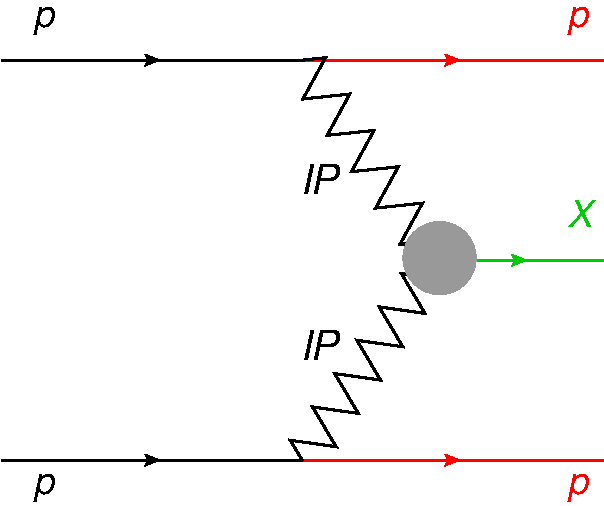
\includegraphics[width=0.92\linewidth]{graphics/introduction/DPE.pdf}\vspace{6pt}%
  \caption{Diagram of D\Pom E process.\\}%
  \label{fig:DPE}\vspace*{-9pt}%
\end{wrapfigure}
%---------------------------

Reaction from Eq.~\eqref{eq:cep} can exhibit purely electromagnetic ($\gamma$-$\gamma$ interaction), mixed ($\gamma$-$\mathcal{O}$ interaction) or purely strong nature ($\mathcal{O}$-$\mathcal{O}$ interaction). The last type is dominant at RHIC energies. In this energy regime it is typically characterized by the lack of hard scale, therefore perturbative QCD cannot be applied and Regge theory~\cite{IntroductionToRegge} is used instead. An object $\mathcal{O}$ does not have unequivocal QCD representation - in Regge formalism it is the so-called ``trajectory`` (\Reg eggeon, \Reg). \Reg eggeon with quantum numbers of vacuum is called ''\Pomeron`` (\Pom) and \Pom-\Pom\ reaction (Fig.~\ref{fig:DPE}) is called ''Double \Pomeron\  Exchange``. %

%---------------------------
\begin{figure}[b!]
\centering
\parbox{0.475\textwidth}{\vspace{-12pt}%
  \centering%
  \hspace*{-18pt}\includegraphics[width=1.3\linewidth]{graphics/introduction/eta_phi.pdf}\vspace*{-15pt}%
  \caption{CEP represented in $\eta$-$\phi$ space.\\}%
  \label{fig:eta_phi}%
}
\quad\quad
\parbox{0.475\textwidth}{%\vspace{-16pt}%
  \centering%
  \includegraphics[width=0.82\linewidth]{graphics/introduction/CEPatSTAR.pdf}%\vspace{6pt}%
  \caption{Central Production event at STAR.\\}\label{fig:CEPatSTAR}%
%   \hspace*{5pt}
}%\vspace*{-25pt}
\end{figure}
%---------------------------

Processes involing \Pomeron\  exchange are referred as diffraction due to cross-section in scattering angle resembling similar shape to instesity pattern of diffracted light. For low values of Mandelstam $t$ (small scattering angles) cross-section takes exponential form\vspace{-2pt}
\begin{equation}
 \frac{d\sigma}{d|t|} \propto e^{-B|t|},
\end{equation}%
where the slope parameter $B$ reflects the transverse size of the interaction region.

Diffractive events have specific property of the ''rapidity gap`` which is an angular region free of hadrons. In \DPE\ two such gaps are present, marked in Fig.~\ref{fig:eta_phi} as $\Delta\eta_{1}$ and $\Delta\eta_{2}$. Figure~\ref{fig:CEPatSTAR} shows the topology of the \DPE\ event on top of the STAR detector, with centrally produced particles marked with green arrows and two forward protons escaping the interaction point inside the beampipe drawn with red arrows.%

\DPE\ is a spin-parity filter - the fact that scattered particles have all quantum numbers unchanged after the interaction, only production of central states satisfying Eq.~\eqref{eq:DPE_IGJPC} is allowed
\begin{equation}\label{eq:DPE_IGJPC}
 I^{G}J^{PC}=0^{+}\textrm{even}^{++}.
\end{equation}%

The lowest order QCD picture of the \Pomeron\ is a pair of oppositely colored gluons (colour singlet). This fact makes the \DPE\ recognized as the gluon-rich environment process in which bound states of gluons (''glueballs``) or hybrid mesons could be produced.

For detailed introduction to the topic of diffraction see Refs.~\cite{pomeronAndQCD,barone}.%\vspace*{-20pt}

% * ** *** **** ***** ****** ******* S E C T I O N ******* ****** ***** **** *** ** *
\section{Physics motivation for the measurement}
STAR collected in 2015 large dataset dedicated for measurement of the Central Diffraction (\DPE\ in particular). Since that year the experiment was enriched with Roman Pot Phase II* subsystem and thus gained possibility of detection of forward scattered protons. It enabled studies of properties of the central state with respect to observables related to exchanged \Pomeron s. No such measurement was performed before at that high c.m.s. energy ($\sqrt{s}=200$~GeV) characterized by small contamination from subleading \Reggeon\ exchanges, which makes it particularly attractive. A brief list of physics issues that can be covered with the study described in this note is briefly introduced below.\vspace{-3pt}%
%
\subsection{\DPE\ differential cross-sections, mass spectrum}

As stated in Sec.~\ref{sec:DPE} \DPE\ is dominantly a soft process whose theoretical description is done mainly using phenomenological tools, thus measurement of differential cross-sections may help to verify various production models.

The main focus is put on the simplest state (and most numerously) produced in \DPE, namely a pair of oppositely charged pions, $\pi^{+}\pi^{-}$. It can be formed either in a non-resonant or resonant mechanism. In the first case the $\pi^{+}\pi^{-}$ continuum can be modelled by the exchange of the off-shell pion between \Pomeron s. Currently there are two models of this reaction on the market~\cite{LSmodel,LSmodel2},~\cite{DurhamModel}. In the second case the \Pomeron s directly couple into resonance (e.g. $f_{2}(1270)$), which then decays to $\pi^{+}\pi^{-}$. Attempts to calculate cross-section for this production mechanism are presented in Ref.~\cite{LSmodel2} and \cite{Schicker}.

Understanding of the mass spectrum in $\pi^{+}\pi^{-}$ channel is important to learn about relative contribution from continuum and resonant production, as well as relative production of resonances. Recognition of resonant states may indicate candidates for low-mass glueballs of $J^{PC}=0^{++}$, however presence of underlaying scalar $q\bar{q}$ states makes this task challenging.

Other channels, like $K^{+}K^{-}$, are also of great interest. Comparison of the cross-sections for production of $\pi^{+}\pi^{-}$ and $K^{+}K^{-}$ gives information about strength of the \Pomeron\ coupling to different quark flavors. Also, structures in $d\sigma/dm$ can be easier attributed to resonances by measuring more than one channel and known branching ratios thereof.

Detection of intact protons scattered at very small angle with respect to the beamline enables determination of the reaction plane which makes the Partial Wave Analysis (PWA) more precise and differential in few more variables. It also allows to look at the the cross-sections more differentially, especially with respect to properties of exchanged \Pomeron s, like carried squared four-momentum $t$, azimuthal separation of \Pomeron s in the transverse plane $\Delta\varphi$ or relative momentum of \Pomeron s $\Delta p_{T}$. The last quantity was proposed to suppress pure $q\bar{q}$ states with respect to these with gluonic content~\cite{DPtFilter}.\vspace{-3pt}

\subsection{Absorption and rescattering effects}

One can imagine in diagram in Fig.~\ref{fig:DPE} additional soft lines e.g. between protons in the initial state, or protons or central state particles in the final state. These so-called rescattering effects (or absorption effects) lead to production of hadrons other than these belonging to central state $X$ hence the diffractive signature of an event in form of rapidity gap is no longer present. Additionally, rescattering may not lead to production of additional hadrons but to redistribution of exclusive cross section over different regions in phase space. Measurement of the probability that the state $X$ will remain exclusive and forward protons will remain intact, in other words the rapidity gap survival probability $S^{2}$, would be valuable ingredient for development of absorption models.\vspace{-3pt}

\subsection{Size of interaction region}

From the measurement of protons in Roman Pots one is able to reconstruct squared four-momenta transferred in proton-\Pomeron\ vertices and determine the differential cross-section $d\sigma/d|t|$. Fit of exponent allows to extract the slope parameter $B$. Knowledge on the slope parameter gives insight to the transverse size of the interaction region.
